\begin{frame}{Vector Operations}
\begin{itemize}
    \item We can add and subtract two vectors $a$ and $b$ of the same size, with the sum denoted $a \pm b$
    \item To get the sum, we add/subtract corresponding entries:
    \begin{align*}
        \begin{bmatrix}
            0\\
            1\\
            1
        \end{bmatrix} \pm \begin{bmatrix}
            9\\
            2\\
            -1
        \end{bmatrix} = \begin{bmatrix}
            0 \pm 9\\
            1 \pm 2\\
            1 \pm (-1)
        \end{bmatrix}
    \end{align*}
    \item Addition of vectors is commutative, associative, and has the zero vector as the neutral element
\end{itemize}
\end{frame}

\begin{frame}{Geometric Interpretation: Addition}
\begin{itemize}
    \item Geometrically, if $a$ and $b$ are vectors, their sum $a+b$ is represented as:
    \begin{figure}[h]
        \centering
        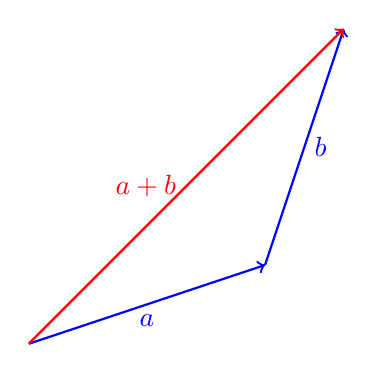
\begin{tikzpicture}
            % Define vectors
            \coordinate (O) at (0,0);
            \coordinate (A) at (3,1);
            \coordinate (B) at (1,3);
            \coordinate (C) at (4,4);
            
            % Draw vectors
            \draw[->, thick, blue] (O) -- (A) node[midway, below] {$a$};
            \draw[->, thick, blue] (A) -- (C) node[midway, right] {$b$};
            \draw[->, thick, red] (O) -- (C) node[midway, left] {$a + b$};
        \end{tikzpicture}
        \caption{Addition of two vectors $a$ and $b$}
        \label{fig:vector-addition}
    \end{figure}
    \item The opposite of a vector $a$, denoted $-a$, is a vector in the opposite direction of $a$
\end{itemize}
\end{frame}

\begin{frame}{Geometric Interpretation: Subtraction}
\begin{itemize}
    \item The representation of $a-b$:
    \begin{figure}[h]
        \centering
        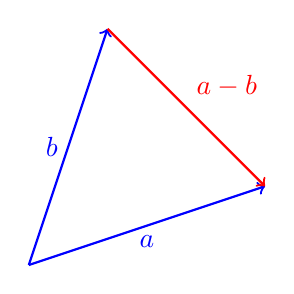
\begin{tikzpicture}
            % Define vectors
            \coordinate (O) at (0,0);
            \coordinate (A) at (3,1);
            \coordinate (B) at (1,3);
            
            % Draw vectors
            \draw[->, thick, blue] (O) -- (A) node[midway, below] {$a$};
            \draw[->, thick, blue] (O) -- (B) node[midway, left] {$b$};
            \draw[->, thick, red] (B) -- (A) node[midway, above right] {$a - b$};
        \end{tikzpicture}
        \caption{Subtraction of two vectors $a$ and $b$}
        \label{fig:vector-subtraction}
    \end{figure}
\end{itemize}
\end{frame}

\begin{frame}{Scalar Multiplication}
\begin{itemize}
    \item We can multiply a vector $a$ by a scalar $\beta$, denoted $\beta a$
    \item $\beta a = (\beta a_1, \beta a_2, \ldots, \beta a_n)$
    \item It is a scaling in the magnitude of the vector $a$:
    \begin{center}
        \begin{tikzpicture}
            % Define vectors
            \coordinate (O) at (0,0);
            \coordinate (A) at (2,1);
            \coordinate (B) at (4,2);
            
            % Draw original vector
            \draw[->, thick, blue] (O) -- (A);
            \node[blue] at (1.2,0.3) {$v$};
            
            % Draw scaled vector
            \draw[->, thick, red] (O) -- (B);
            \node[red] at (2.5,1.3) {$\beta v$};
            
            % Dotted lines for visualization
            \draw[dashed, gray] (A) -- (B);
        \end{tikzpicture}
    \end{center}
    \item Scalar multiplication is associative and distributive
\end{itemize}
\end{frame}

%  Elementwise multiplicatio ------

\begin{frame}{Element-wise Multiplication}
\begin{itemize}
    \item For two $n$-vectors $a$ and $b$, the element-wise multiplication $a \circ b$ produces a vector where each component is the product of corresponding elements
    \item Formally:
    \begin{align*}
        a \circ b = (a_1 b_1, a_2 b_2, \ldots, a_n b_n)
    \end{align*}
    \item The symbol $\circ$ or $\star$ denotes \textit{element-wise} or \textit{Hadamard} multiplication
\end{itemize}
\end{frame}
\begin{frame}
    \begin{itemize}
        \item Example: 
    \begin{align*}
        (0, -1, 2) \circ (1, -1, \frac{1}{2}) = (0 \cdot 1, (-1) \cdot (-1), 2 \cdot \frac{1}{2}) = (0, 1, 1)
    \end{align*}
        \item Element-wise multiplication is not commutative, i.e., $a \circ b \neq b \circ a$ in general
        \item However, it is associative, i.e., $(a \circ b) \circ c = a \circ (b \circ c)$
        \item It is distributive over vector addition, i.e., $a \circ (b + c) = a \circ b + a \circ c$
        \item \textbf{Note:} This operation is intensively used in NumPy and machine learning for vectorization.
    \end{itemize}
\end{frame}

\begin{frame}{Transpose and Linear Combinations}
\begin{itemize}
    \item \textbf{Transpose:} For an $(n,1)$-vector $x$, its transpose $x^T$ is a $(1,n)$-vector
    \item Properties of transpose:
    \begin{itemize}
        \item $(x^T)^T = x$  (Transpose of transpose is the original vector)
        \item $(\beta x)^T = \beta x^T$ for a scalar $\beta$
        \item $(x + y)^T = x^T + y^T$ for vectors $x$ and $y$
    \end{itemize}
    \item \textbf{Linear combination:} A linear combination of vectors $x_1, x_2, \ldots, x_k$ with scalars $\alpha_1, \alpha_2, \ldots, \alpha_k$ is:
     \begin{align*}
        y = \alpha_1 x_1 + \alpha_2 x_2 + \ldots + \alpha_k x_k
    \end{align*}
    \item This is a vector formed by scaling and adding the vectors $x_i$.
    
\end{itemize}
\end{frame}

\begin{frame}
    \begin{itemize}
        \item Example: For $x_1 = \begin{bmatrix} 1 \\ 2 \end{bmatrix}$, $x_2 = \begin{bmatrix} 3 \\ 4 \end{bmatrix}$, and $\alpha_1 = 2$, $\alpha_2 = -1$:
    \begin{align*}
        y = 2 \begin{bmatrix} 1 \\ 2 \end{bmatrix} - 1 \begin{bmatrix} 3 \\ 4 \end{bmatrix} = \begin{bmatrix} 2 \\ 4 \end{bmatrix} - \begin{bmatrix} 3 \\ 4 \end{bmatrix} = \begin{bmatrix} -1 \\ 0 \end{bmatrix}
    \end{align*}
        \item The result $y$ is a vector in the same dimension  as $x_1$ and $x_2$.
        \item Linear combinations are fundamental in linear algebra, forming the basis for \textbf{vector spaces}.
    \end{itemize}
\end{frame}



